\chapter{結果と考察}
共振周波数を変化させるためには、共振器の大きさを変化させる方法と、と内部に誘電体あるいは導体を挿入する方法がある。共振器自体の大きさを変化させて共振周波数を調整する方法では、全ての辺の長さの比を一定にしなければ、内部の電磁場分布が大きく変化してしまい、大きさの変化とともに試料設置位置も変動させる必要が出てくるが試料設置位置を動かすことは現実的ではない。また、全ての方向で大きさの比を保ちながら共振器の大きさを変化させるためにはかなり高度なギミックが必要となり、これも現実的ではない。そのため今回は内部に誘電体を挿入することによって、共振周波数を現象させるという方法で実現を目指す。


\section{誘電体挿入による影響}
まず、誘電体挿入による影響を調べるための検証を行った。
大きさが同じ共振器(基本モード$TE101$)を用いて、誘電率9の誘電体(サファイア)を下図のように

\begin{enumerate}
  \item 共振器よりも小さいサイズで位置のみを変化させたモデル
  \item 共振器と同じサイズで徐々に挿入していくモデル
\end{enumerate}

の2つの場合で検証を行った。

\vspace{10 mm}

\begin{figure}[h]
  \begin{center}
    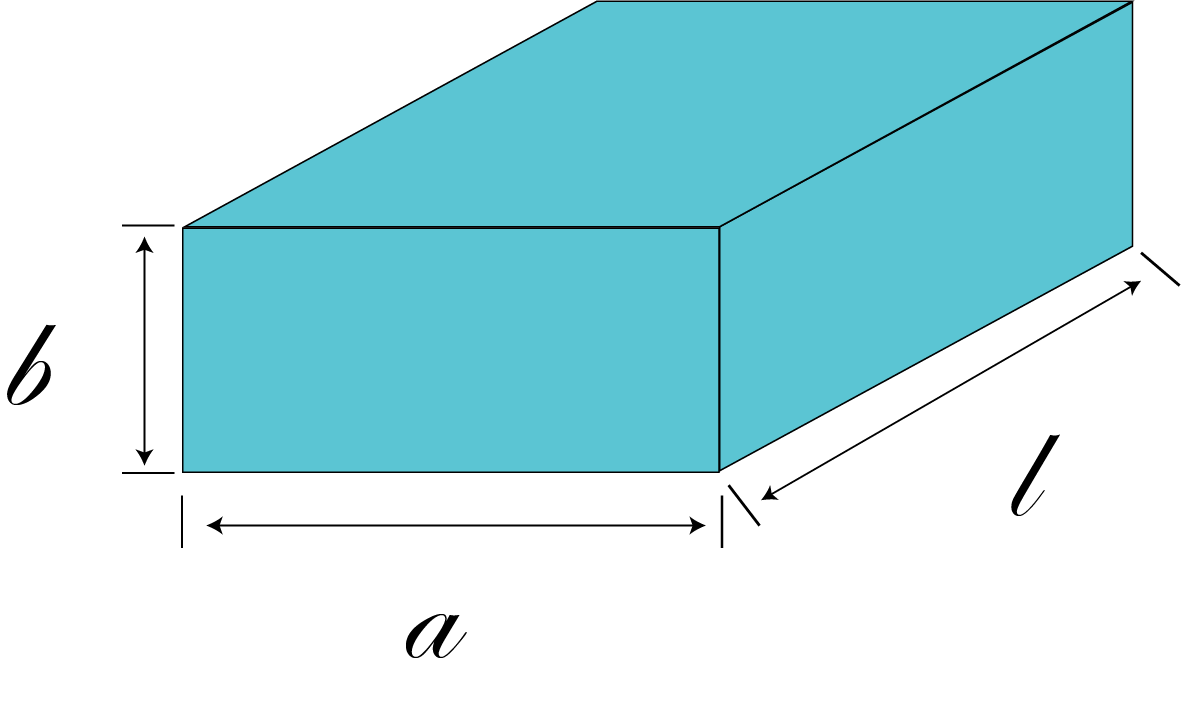
\includegraphics[width=5cm]{./image/空洞共振器.png}
    \caption{方形空洞共振器}
    \label{fig:Cavity}
  \end{center}
\end{figure}

\vspace{10 mm}

\begin{figure}[h]
  \begin{center}
    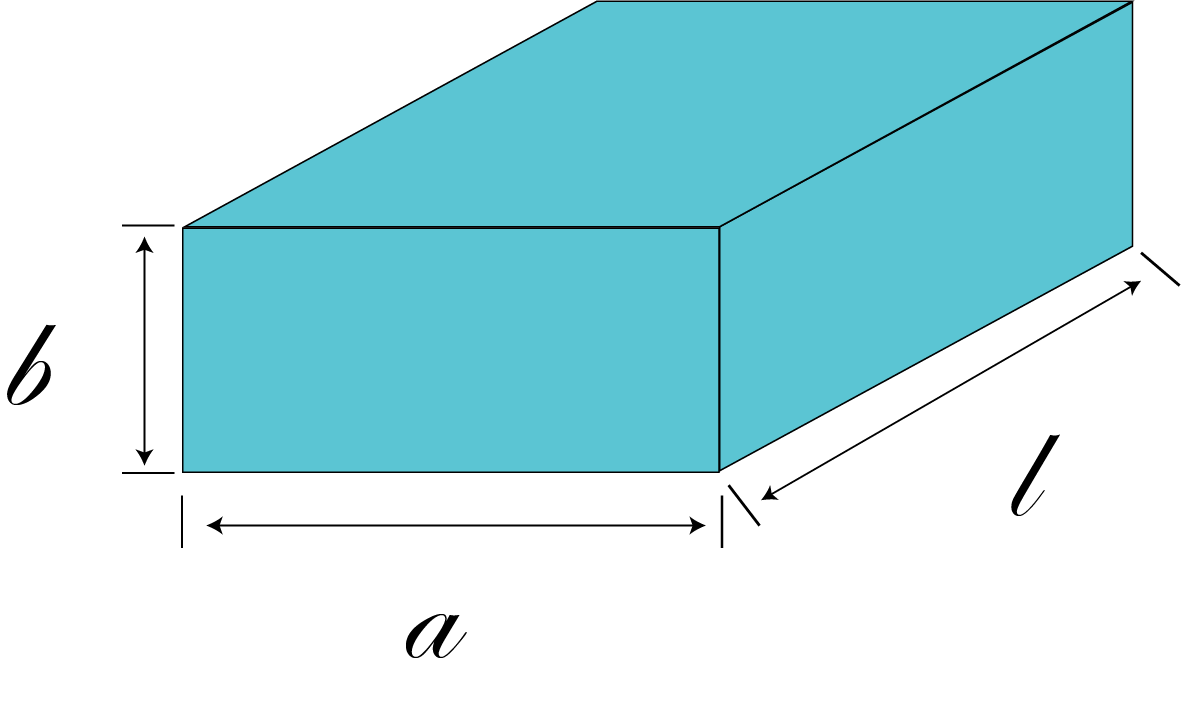
\includegraphics[width=5cm]{./image/空洞共振器.png}
    \caption{方形空洞共振器}
    \label{fig:Cavity}
  \end{center}
\end{figure}

\subsection{結果}

\vspace{10 mm}

\begin{figure}[h]
  \begin{center}
    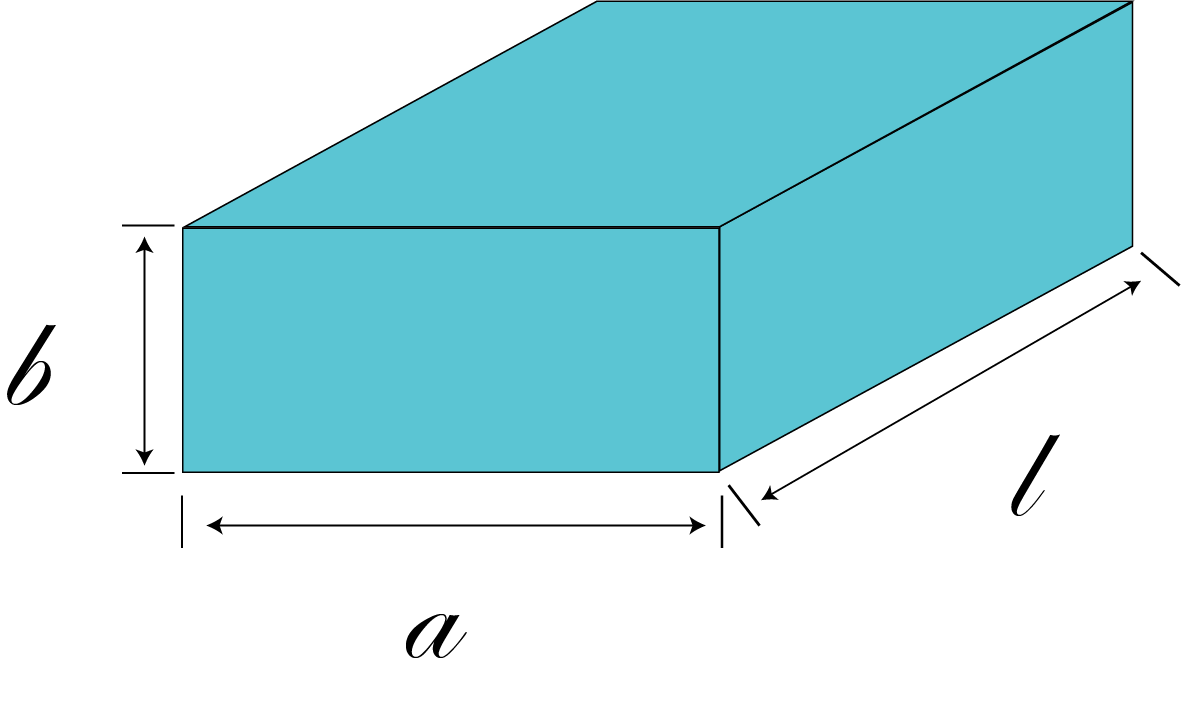
\includegraphics[width=5cm]{./image/空洞共振器.png}
    \caption{方形空洞共振器}
    \label{fig:Cavity}
  \end{center}
\end{figure}

\subsection{考察}


\section{提案するモデル}
この結果を受けて今回は以下のようなモデルを提案する。
\subsection{設計}
\vspace{10 mm}

\begin{figure}[h]
  \begin{center}
    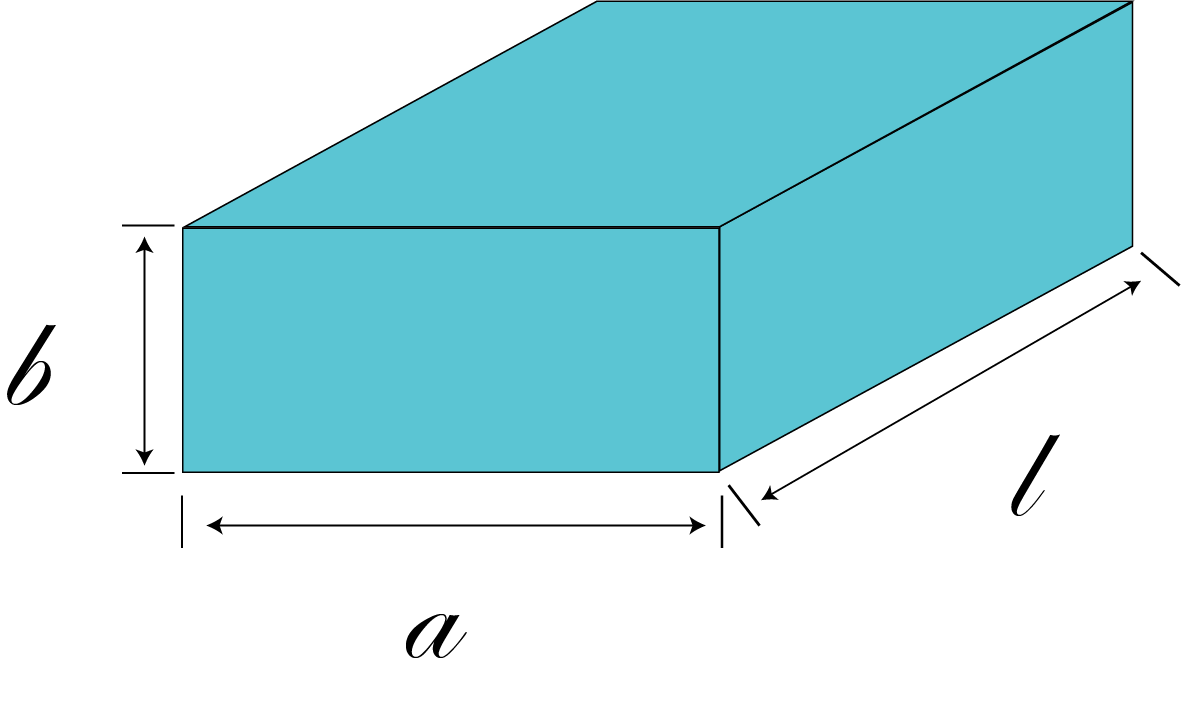
\includegraphics[width=5cm]{./image/空洞共振器.png}
    \caption{方形空洞共振器}
    \label{fig:Cavity}
  \end{center}
\end{figure}

\vspace{10 mm}

\begin{figure}[h]
  \begin{center}
    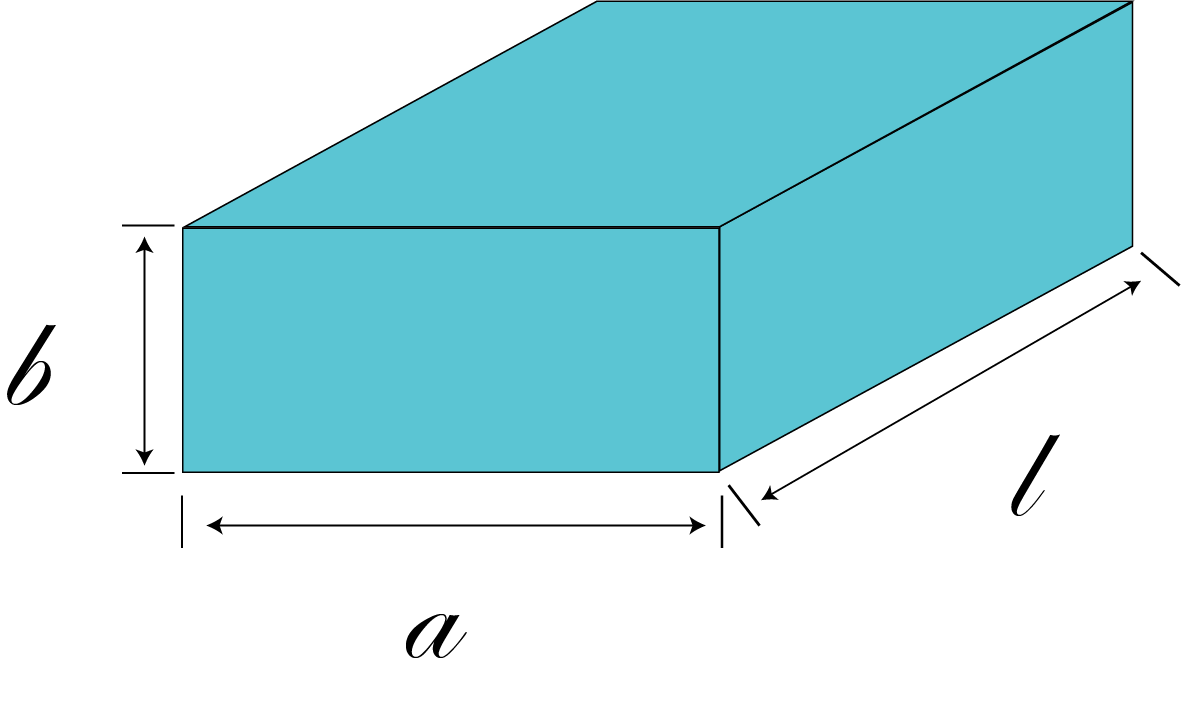
\includegraphics[width=5cm]{./image/空洞共振器.png}
    \caption{方形空洞共振器}
    \label{fig:Cavity}
  \end{center}
\end{figure}

\vspace{10 mm}

\begin{figure}[h]
  \begin{center}
    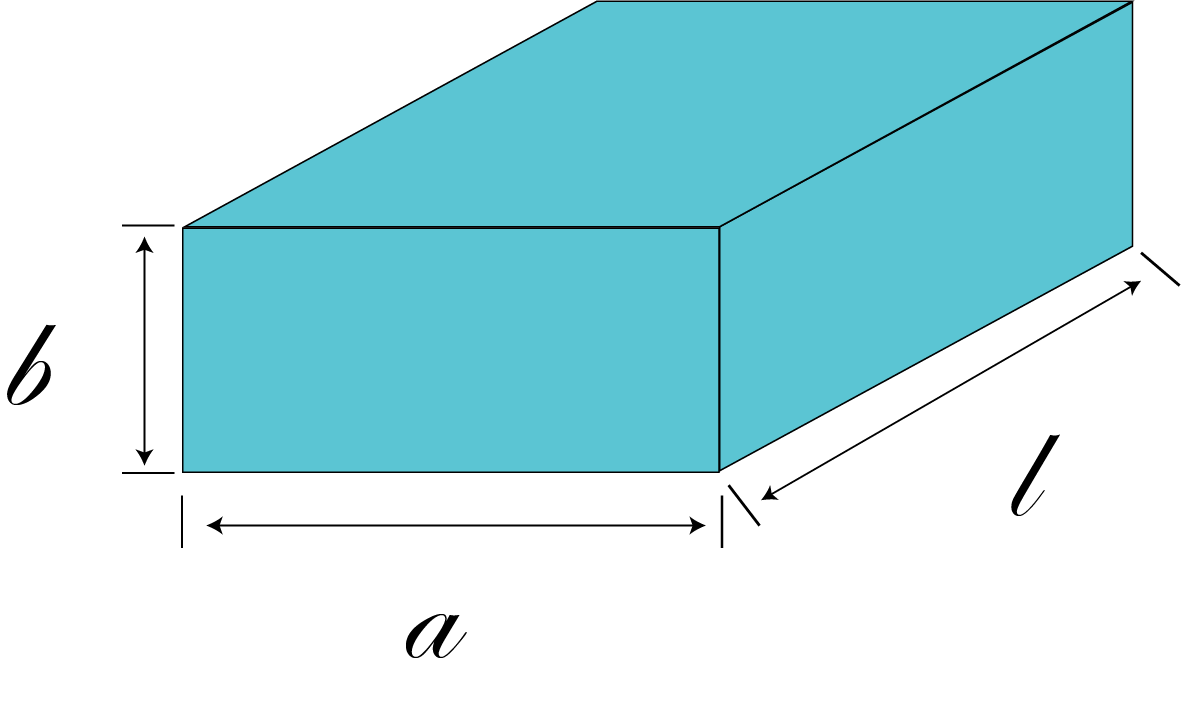
\includegraphics[width=5cm]{./image/空洞共振器.png}
    \caption{方形空洞共振器}
    \label{fig:Cavity}
  \end{center}
\end{figure}

\vspace{10 mm}

\begin{figure}[h]
  \begin{center}
    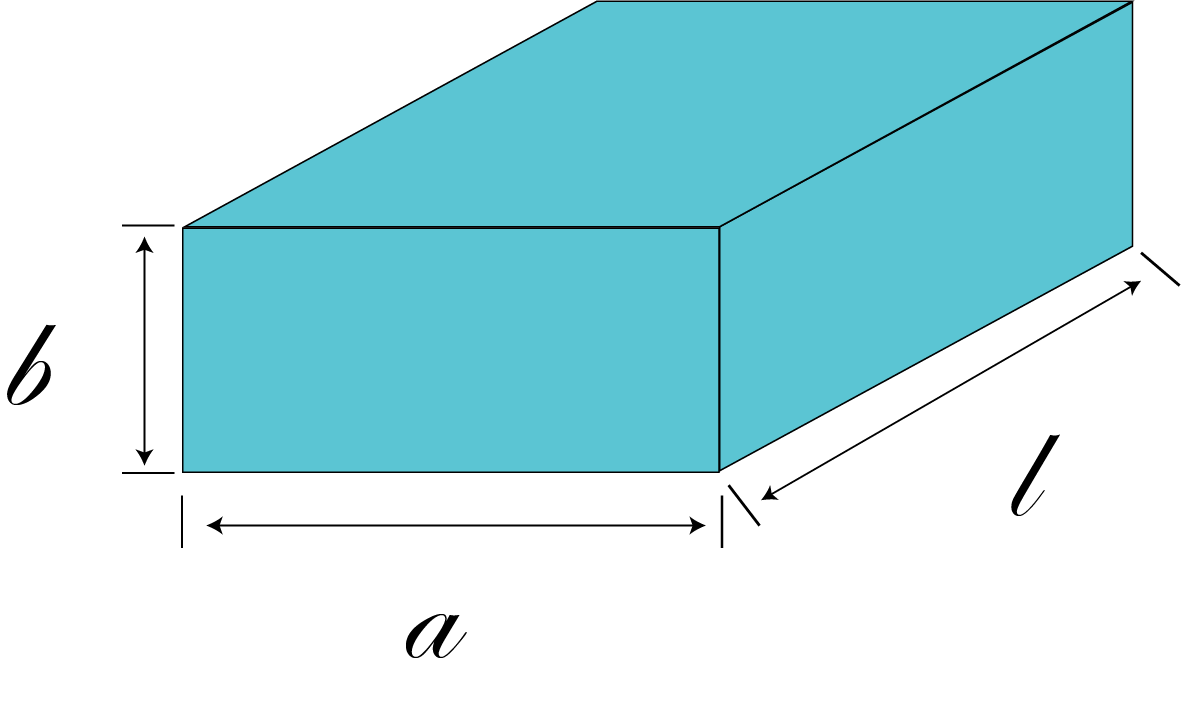
\includegraphics[width=5cm]{./image/空洞共振器.png}
    \caption{方形空洞共振器}
    \label{fig:Cavity}
  \end{center}
\end{figure}

\subsection{基本性質}
\vspace{10 mm}

\begin{figure}[h]
  \begin{center}
    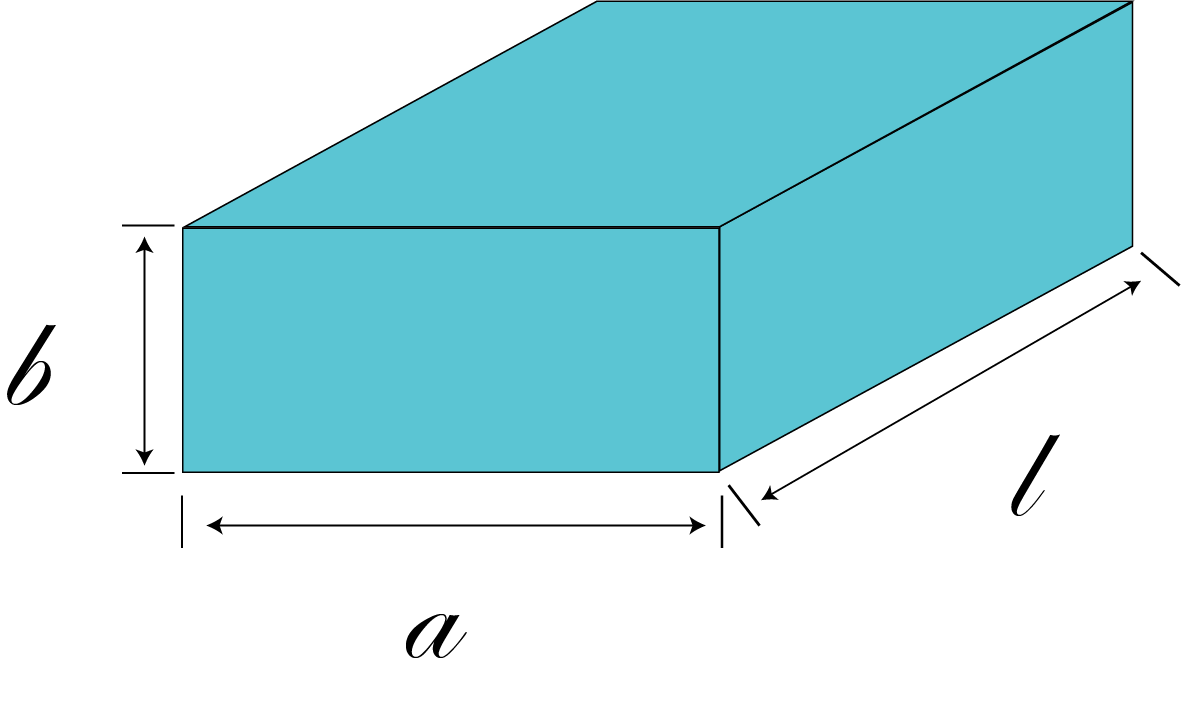
\includegraphics[width=5cm]{./image/空洞共振器.png}
    \caption{方形空洞共振器}
    \label{fig:Cavity}
  \end{center}
\end{figure}

\vspace{10 mm}

\begin{figure}[h]
  \begin{center}
    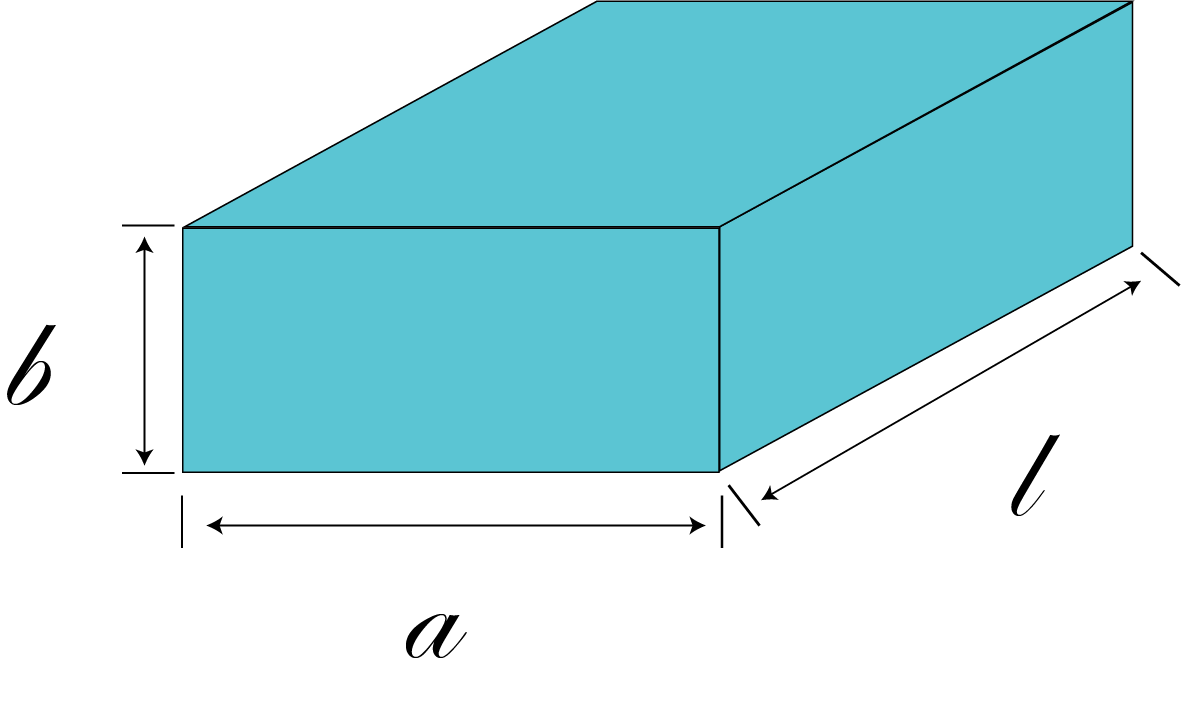
\includegraphics[width=5cm]{./image/空洞共振器.png}
    \caption{方形空洞共振器}
    \label{fig:Cavity}
  \end{center}
\end{figure}

\vspace{10 mm}

\begin{figure}[h]
  \begin{center}
    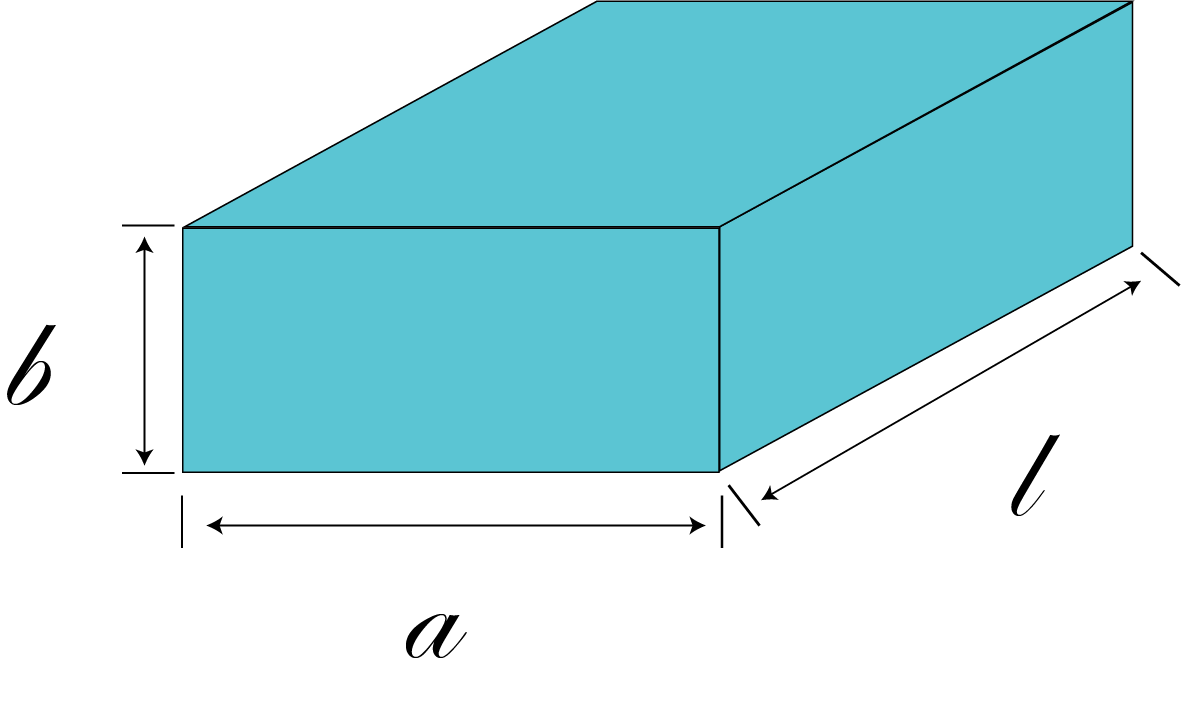
\includegraphics[width=5cm]{./image/空洞共振器.png}
    \caption{方形空洞共振器}
    \label{fig:Cavity}
  \end{center}
\end{figure}

\subsection{誘電体挿入時の共振周波数変化}

\vspace{10 mm}

\begin{figure}[h]
  \begin{center}
    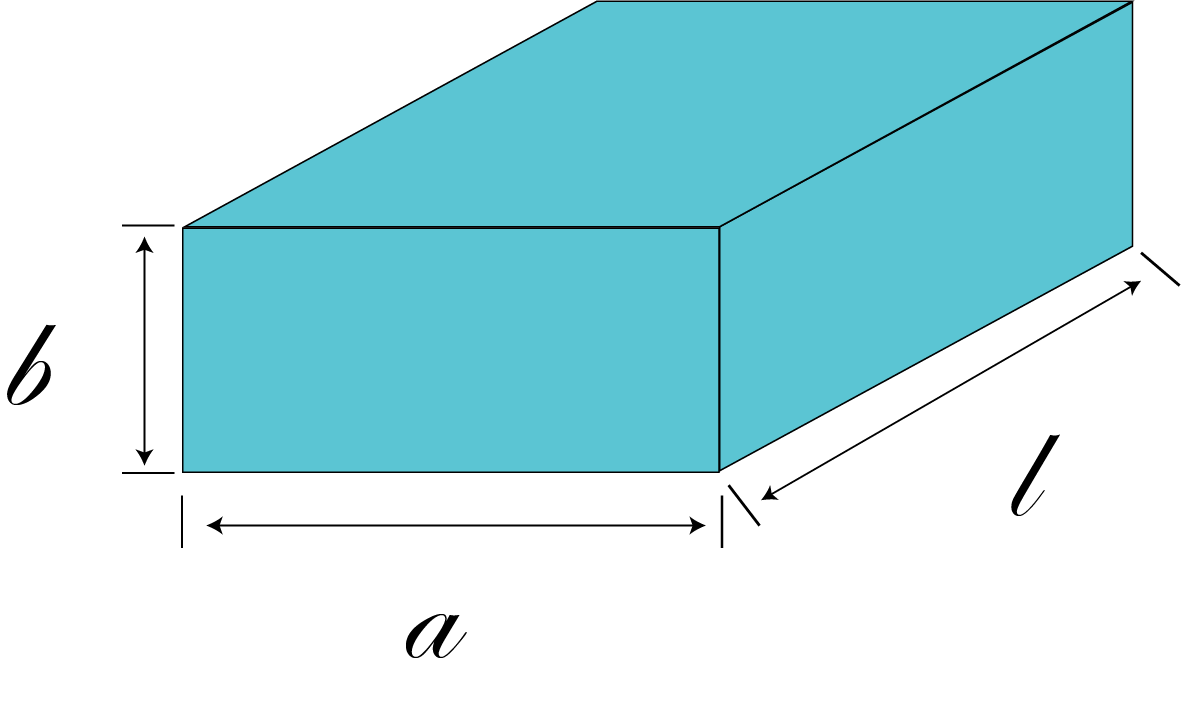
\includegraphics[width=5cm]{./image/空洞共振器.png}
    \caption{方形空洞共振器}
    \label{fig:Cavity}
  \end{center}
\end{figure}

\subsection{考察}
